%%% Hlavní soubor. Zde se definují základní parametry a odkazuje se na ostatní části. %%%

% Meta-data o práci (je nutno upravit)
\input metadata.tex

% Vygenerujeme metadata ve formátu XMP pro použití balíčkem pdfx
\input xmp.tex

%% Verze pro jednostranný tisk:
% Okraje: levý 40mm, pravý 25mm, horní a dolní 25mm
% (ale pozor, LaTeX si sám přidává 1in)
%\documentclass[12pt,a4paper]{report}
%\setlength\textwidth{145mm}
%\setlength\textheight{247mm}
%\setlength\oddsidemargin{15mm}
%\setlength\evensidemargin{15mm}
%\setlength\topmargin{0mm}
%\setlength\headsep{0mm}
%\setlength\headheight{0mm}
%% \openright zařídí, aby následující text začínal na pravé straně knihy
%\let\openright=\clearpage

%% Pokud tiskneme oboustranně:
% \documentclass[12pt,a4paper,twoside,openright]{report}
% \setlength\textwidth{145mm}
% \setlength\textheight{247mm}
% \setlength\oddsidemargin{14.2mm}
% \setlength\evensidemargin{0mm}
% \setlength\topmargin{0mm}
% \setlength\headsep{0mm}
% \setlength\headheight{0mm}
% \let\openright=\cleardoublepage

% Pokud práci odevzdáváme pouze elektronicky, vypadají lépe symetrické okraje
\documentclass[12pt,a4paper]{report}
\setlength\textwidth{145mm}
\setlength\textheight{247mm}
\setlength\oddsidemargin{10mm}
\setlength\evensidemargin{10mm}
\setlength\topmargin{0mm}
\setlength\headsep{0mm}
\setlength\headheight{0mm}
\let\openright=\clearpage

%% Vytváříme PDF/A-2u
\usepackage[a-2u]{pdfx}

%% Přepneme na českou sazbu a fonty Latin Modern
\usepackage[czech]{babel}
\usepackage{lmodern}

% Pokud nepouživáme LuaTeX, je potřeba ještě nastavit kódování znaků
\usepackage{iftex}
\ifpdftex
\usepackage[utf8]{inputenc}
\usepackage[T1]{fontenc}
\usepackage{textcomp}
\fi

%%% Další užitečné balíčky (jsou součástí běžných distribucí LaTeXu)
\usepackage{amsmath}        % rozšíření pro sazbu matematiky
\usepackage{amsfonts}       % matematické fonty
\usepackage{amsthm}         % sazba vět, definic apod.
\usepackage{bm}             % tučné symboly (příkaz \bm)
\usepackage{booktabs}       % lepší vodorovné linky v tabulkách
\usepackage{caption}        % umožní definovat vlastní popisky plovoucích objektů
\usepackage{csquotes}       % uvozovky závislé na jazyku
\usepackage{dcolumn}        % vylepšené zarovnání sloupců tabulek
\usepackage{floatrow}       % umožní definovat vlastní typy plovoucích objektů
\usepackage{graphicx}       % vkládání obrázků
\usepackage{icomma}         % inteligetní čárka v matematickém módu
\usepackage{indentfirst}    % zavede odsazení 1. odstavce kapitoly
\usepackage[nopatch=item]{microtype}  % mikrotypografická rozšíření
\usepackage{paralist}       % lepší enumerate a itemize
\usepackage[nottoc]{tocbibind} % zajistí přidání seznamu literatury,
                            % obrázků a tabulek do obsahu
\usepackage{xcolor}         % barevná sazba

% Balíček hyperref, kterým jdou vyrábět klikací odkazy v PDF,
% ale hlavně ho používáme k uložení metadat do PDF (včetně obsahu).
% Většinu nastavítek přednastaví balíček pdfx.
\hypersetup{unicode}
\hypersetup{breaklinks=true}

% Balíčky pro sazbu informatických prací
\usepackage{algpseudocode}  % součást balíčku algorithmicx
\usepackage[Algoritmus]{algorithm}
\usepackage{fancyvrb}       % vylepšené prostředí verbatim
\usepackage{listings}       % zvýrazňování syntaxe zdrojových textů

% Cleveref může zjednodušit odkazování, ale jeho užitečnost pro češtinu
% je minimalní, protože nezvládá skloňování.
% \usepackage{cleveref}

% Formátování bibliografie (odkazů na literaturu)
% Detailní nastavení můžete upravit v souboru macros.tex.
%
% POZOR: Zvyklosti různých oborů a kateder se liší. Konzultujte se svým
% vedoucím, jaký formát citací je pro vaši práci vhodný!
%
% Základní formát podle normy ISO 690 s číslovanými odkazy
\usepackage[natbib,style=iso-numeric,sorting=none]{biblatex}
% ISO 690 s alfanumerickými odkazy (zkratky jmen autorů)
%\usepackage[natbib,style=iso-alphabetic]{biblatex}
% ISO 690 s citacemi tvaru Autor (rok)
%\usepackage[natbib,style=iso-authoryear]{biblatex}
%
% V některých oborech je běžnější obyčejný formát s číslovanými odkazy
% (sorting=none říká, že se bibliografie má řadit podle pořadí citací):
%\usepackage[natbib,style=numeric,sorting=none]{biblatex}
% Číslované odkazy, navíc se [1,2,3,4,5] komprimuje na [1-5]
%\usepackage[natbib,style=numeric-comp,sorting=none]{biblatex}
% Obyčejný formát s alfanumerickými odkazy:
%\usepackage[natbib,style=alphabetic]{biblatex}

% Z tohoto souboru se načítají položky bibliografie
\addbibresource{literatura.bib}

% Definice různých užitečných maker (viz popis uvnitř souboru)
\input macros.tex

%%% Titulní strana a různé povinné informační strany
\begin{document}
%%% Titulní strana práce a další povinné informační strany

%%% Nápisy na přední straně desek
%%% Pokud je práce ve slovenštině, desky mají být česky.

% Desky obvykle nesázíme, ale pokud je chcete přidat, změnte \iffalse na \iftrue
\iffalse

\pagestyle{empty}
\hypersetup{pageanchor=false}
\begin{center}

\large
Univerzita Karlova

\medskip

Matematicko-fyzikální fakulta

\vfill

{\huge\bf\ThesisTypeTitle}

\vfill

{\huge\bf\ThesisTitle\par}

\vfill
\vfill

\hbox to \hsize{\YearSubmitted\hfil \ThesisAuthor}

\end{center}

\newpage\openright
\setcounter{page}{1}

\fi

%%% Titulní strana práce
%%% Pokud je práce ve slovenštině, tato strana zůstává česky.

\pagestyle{empty}
\hypersetup{pageanchor=false}

\begin{center}

\centerline{\mbox{
\includegraphics[width=166mm]{img/logo-cs.pdf}}}

\vspace{-8mm}
\vfill

{\bf\Large\ThesisTypeTitle}

\vfill

{\LARGE\ThesisAuthor}

\vspace{15mm}

{\LARGE\bfseries\ThesisTitle\par}

\vfill

\Department

\vfill

{
\centerline{\vbox{\halign{\hbox to 0.45\hsize{\hfil #}&\hskip 0.5em\parbox[t]{0.45\hsize}{\raggedright #}\cr
Vedoucí \ThesisTypeGenitive{} práce:&\Supervisor \cr
\ifx\ThesisType\TypeRig\else
\noalign{\vspace{2mm}}
Studijní program:&\StudyProgramme \cr
\fi
}}}}

\vfill

Praha \YearSubmitted

\end{center}

\newpage

%%% Strana s čestným prohlášením k práci
%%% Pokud je práce ve slovenštině, tato strana zůstává česky.

\openright
\hypersetup{pageanchor=true}
\vglue 0pt plus 1fill

\noindent
Prohlašuji, že jsem tuto \ThesisTypeAccusative{} práci vypracoval(a) samostatně a výhradně
s~použitím citovaných pramenů, literatury a dalších odborných zdrojů.
Beru na~vědomí, že se na moji práci vztahují práva a povinnosti vyplývající
ze zákona č. 121/2000 Sb., autorského zákona v~platném znění, zejména skutečnost,
že Univerzita Karlova má právo na~uzavření licenční smlouvy o~užití této
práce jako školního díla podle §60 odst. 1 autorského zákona.

\vspace{10mm}

\hbox{\hbox to 0.5\hsize{%
V \hbox to 6em{\dotfill} dne \hbox to 6em{\dotfill}
\hss}\hbox to 0.5\hsize{\dotfill\quad}}
\smallskip
\hbox{\hbox to 0.5\hsize{}\hbox to 0.5\hsize{\hfil Podpis autora\hfil}}

\vspace{20mm}
\newpage

%%% Poděkování

\openright

\noindent
\Dedication

\newpage

%%% Povinná informační strana práce

\openright
{\InfoPageFont

\vtop to 0.5\vsize{
\setlength\parindent{0mm}
\setlength\parskip{5mm}

Název práce:
\ThesisTitle

Autor:
\ThesisAuthor

\DeptType:
\Department

Vedoucí \ThesisTypeGenitive{} práce:
\Supervisor, \SupervisorsDepartment

Abstrakt:
\Abstract

Klíčová slova:
{\def\sep{\unskip, }\ThesisKeywords}

\vfil
}

\vtop to 0.49\vsize{
\setlength\parindent{0mm}
\setlength\parskip{5mm}

Title:
\ThesisTitleEN

Author:
\ThesisAuthor

\DeptTypeEN:
\DepartmentEN

Supervisor:
\Supervisor, \SupervisorsDepartmentEN

Abstract:
\AbstractEN

Keywords:
{\def\sep{\unskip, }\ThesisKeywordsEN}

\vfil
}

}

\newpage

%%% Další stránky budeme číslovat, což LaTeX zařídí sám na začátku kapitoly


%%% Strana s automaticky generovaným obsahem práce

\tableofcontents

%%% Jednotlivé kapitoly práce jsou pro přehlednost uloženy v samostatných souborech
\chapter*{Úvod}
\addcontentsline{toc}{chapter}{Úvod}

Následuje několik ukázkových kapitol, které doporučují, jak by se
měla bakalářská práce sázet. Primárně popisují použití \TeX{}ové
šablony, ale obecné rady poslouží dobře i~uživatelům jiných
systémů.

\chapter{Evoluční Algoritmy}

\xxx{Nějaké povídání o evolučních algoritmech.}

\section{Zakládní definice}
V této sekci bychom chtěli definovat některé užitečné pojmy, ukázat základní komponenty evolučních algorimtů a zároveň vysvětlit, jakou hrají roli při návrhu a běhu algoritmu.

\subsection{Gen a Jedinec}
Gen představuje jedno řešení pro daný problém. Je důležité zvolit vhodné kódování tohoto řešení. Holland si ve svém původním návrhu evolučního algoritmu představoval, že každé řešení bude binárně kódováno (holland citace), ale později se ukázalo, že je možné dosáhnout lepších výsledků, když kódováním reprezentujeme jakési stavební bloky daného řešení \citet{HeadlessChicken}.

Jedincem pak myslíme zastoupení genu v populaci.

\subsection{Populace a Generace}
Populace je seznam jedinců. Ze začátku běhu algoritmu populaci většinou naplníme jedinci s náhodnými geny a postupnou aplikací genetických operátorů v ní budeme vyvíjet lepší a lepší řešení. Generace představuje stav populace v konkrétním čase.

\subsection{Genetické operátory}
Genetické operátory jsou funkce, které můžeme aplikovat na celou populaci s cílem vybrat lepší jedince do další generace. Pomocí těchto operátorů můžeme vyvažovat exploraci a exploataci algoritmu a zároveň celou populaci směřovat k optimálnímu řešení (možná citace).

V kontextu genetických operátorů budeme často mluvit o rodičích a potomcích. Rodiči myslíme ty jedince, které se v populaci nachází před aplikací genetických operátorů, potomky pak ty, které se nachazí po aplikaci, neboli v další generaci. 

\subsection{Křížení}
Křižení je genetický operátor, kterým ze dvou nebo více jedinců (rodičů) můžeme vytvořit nového jedince (potomka), který strukturou připomíná oba všechny svoje rodiče. Tento proces je inspirován biologickou reprodukcí, kde potomci zdědí vlastnosti obou rodičů, což může vést k vyšší genetické variabilitě v populaci. Je důležité, aby nový potomek nebyl pouze náhodnou kombinací částí genů svých rodičů, ale aby křížení opravdu dávalo z hlediska struktury smysl (headless chicken citace).

\subsection{Mutace}
Mutace je genetický operátor, který může měnit náhodné části genu. Od křížení se liší hlavně tím, že je nezávislá na ostatních genech v populaci. Význam mutací spočívá v udržení genetické diverzity populace, což je zásadní pro průzkum širšího prostoru řešení a předcházení předčasné konvergenci k suboptimálním řešením.

\subsection{Fitness}
Fitness je funkce, zde označená písmenem $f$, taková že $f: G \rightarrow \R$ kde $G$ představuje množinu všech možných genů. V problémech, které budeme chtít řešit evolučními algoritmy, se funkci $f$ obvykle snažíme maximalizovat. Jinými slovy, hledáme takový gen $g^* \in G$, že 
$$g^* = argmax_{g \in G} f(g)$$

Fitness funkce nabízí měřitelnou kvalitu daného genu a pomáhají algoritmu rozlišovat mezi více a méně vhodnými jedinci. Při návrhu fitness funkce je však nutné být opatrný, aby se předešlo běžným problémům, jako je předčasná konvergence nebo uváznutí v lokálních maximech. Není neobvyklé, že do fitness funkce je zahrnuto více různých komponent, které do výsledné hodnoty přispivají různými vahami. Tímto způsobem můžeme lépe rozlišit kvalitní řešení od těch nekvalitních a poskytnout algoritmu více informací pro efektivní průzkum prostoru řešení. V praxi to může znamenat, že vedle hlavního kritéria, jako je například výkon nebo efektivita, mohou být do fitness funkce zahrnuty i sekundární kritéria, jako je cena, estetičnost nebo další meta-heuristiky, které mohou pomoci při hledání optimálního řešení.

\subsection{Selekce}
Selekce, nebo také environmentální selekce, je genetický operátor, který simuluje proces přírodního výběru. Tento operátor přiřazuje jednotlivým jedincům jejich schopnosti přežívat a reprodukovat se na základě jejich fitness. Ti nejúspěšnější jedinci jsou vybíráni pro reprodukci, zatímco ti méně úspěšní jsou buď eliminováni nebo mají menší šanci přispět svými geny do další generace. Díky selekci se algoritmus soustředí na oblasti vyhledávacího prostoru s vysokým potenciálem, což vede k rychlejší a konvergenci k optimálním řešením. 

V kontextu selekce se často mluví o $(\mu + \lambda)$ a $(\mu, \lambda)$ selekci. 

$(\mu + \lambda)$ selekce spočívá v tom, že z $\mu$ rodičů generujeme $\lambda$ potomků. Tyto potomky následně spojíme s původními rodiči a z této kombinované skupiny vybereme nejlepších $\mu$ jedinců pro další generaci. Tento přístup zajišťuje zachování nejlepších genetických vlastností z předešlých generací a poskytuje pojistku proti ztrátě kvalitních genů v případě, že nová generace by byla průměrně horší než její předchůdce. (citace kniha)

Na druhou stranu, $(\mu, \lambda)$ selekce vychází z principu, kde $\mu$ rodičů generuje $\lambda$ potomků, ale pouze tito potomci postupují do další generace, což znamená úplné nahrazení původní populace. Tento proces, při němž jsou všichni rodiče nahrazení, pomáhá efektivněji překonávat lokální minima prostoru řešení, což je obzvláště cenné v situacích, kde prostor řešení obsahuje mnoho lokálních minim. (citace kniha)

\section{Evoluční algoritmus}

Příklad návrhu jednoduchého evolučního algoritmu může můžeme vidět v algoritmu 1.

\begin{algorithm}
\caption{Jednoduchý evoluční algoritmus}
\begin{algorithmic}[1]  % [1] způsobí, že číslujeme kroky algoritmu
\Function{EA}{Selekce, Křížení, Mutace, Fitness}
	\State $p \gets \mbox{náhodně inicializujeme populaci}$
    \State $f \gets Fitness(p_1), \dots, Fitness(p_n)$ \Comment{ohodnotíme fitness pro každého jedince}
	\While{$\mbox{není dosaženo zastavovací kriterium}$}
		\State $p \gets \mbox{Selekce}(p, f)$
		\State $p \gets \mbox{Křížení}(p)$
		\State $p \gets \mbox{Mutace}(p)$
        \State $f \gets \mbox{Fitness}(p_1), \dots, Fitness(p_n)$
    \EndWhile
    \State Vrátíme nejlepšího jedince z $p$
\EndFunction
\end{algorithmic}
\end{algorithm}




\section{Přiklady}

V této části bychom chtěli ukázat, jak lze navrhnout evoluční algoritmus pro řešení některých vybraných netriviálních problémů.

\subsection{Problém Batohu}

Problém batohu je generalizace mnoha industriálních problémů (citace knížka). Představme si, že se balíme třeba na několikadenní túru do hor a s sebou bychom si chtěli zabalit batůžek. Chtěli bychom s sebou mít co nejužitečnější věci, ale zároveň si nemůžeme vzít všechno, protože bychom to neunesli. Problém batohu spočívá v tom, jak si vybrat věci, které si s sebou zabalíme, tak abychom maximalizovali užitek a zároveň se vešli do našeho stanoveného limitu.

Formálněji se tento problém definuje následovně. Je dána množina $n$ předmětů s hmotnostmi $h_1, \dots, h_n \in \N$, cenami $c_1, \dots, c_n \in \N$ a maximální hmotnost $H \in \N$. Hledáme takovou podmnožinu $p \subseteq \{1, \dots n\}$, pro kterou platí, že $\sum_{i \in P} h_i \leq H$ a zároveň $\sum_{i \in P} c_i$ je co největší.

Jako ilustrační řešení tomuto problému jsme navrhli tyto evoluční operátory a reprezentace:
\begin{itemize}
    \item Gen bude řetězec $\alpha \in \{0,1\}^n$, kde $\alpha_i$ ($i$-tý prvek z řetězce) značí, zda jsme se rozhodli vybrat $i$-tý prvek do množiny $p$ nebo ne.
    \item Jako selekci jsme zvolili turnajovou selekci. Při turnajové selekci náhodně zvolíme $k$ jedinců z populace. Z těchto $k$ jedinců postupuje do další generace pouze ten s nejvyšší fitness. Tímto způsobem můžeme
    \item Jako mutaci jsem zvolili jednobodové křížení. To v praxi znamená, že pro dva jedince, které spolu chceme zkřížit
    \item Fitness funkce $f$ v tomto případě bude $f(\alpha) = \sum_{i=1}^n \alpha_i \cdot \c_i$ pokud $\sum_{i=1}^n \alpha_i \cdot h_i < W$ jinak $0$
\end{itemize}

Výsledky běhu takového algoritmu můžeme vidět ve obrázku 1.1

\xxx{Měli bych uvéšt více příkladů?}

\chapter{Hra PolyBridge}

Poly Bridge je logická simulovaná hra, která byla vyvinuta nezávislým vývojářským týmem Dry Cactus. Hráči mají za úkol navrhovat mosty, které musí odolat zátěži projíždějících vozidel a zároveň splňovat omezení daná rozpočtem a dostupnými materiály. Díky svému základu v realistické fyzice nabízí Poly Bridge možnost experimentovat s různými stavebními technikami a materiály.

Poly Bridge odráží řadu reálných principů stavitelství mostů. Stejně jako ve skutečnosti, mosty ve hře vyžadují pečlivé plánování a zohlednění sil, které na ně působí. Tyto síly zahrnují napětí, tlak, ohyb a torzi. Hra tedy poskytuje hráčům intuitivní pochopení těchto principů prostřednictvím připravených výzev a následné simulace. K tomu hráči využívají různé materiály jako jsou dřevo, ocel a lano, přičemž každý materiál má specifické vlastnosti a omezení vzhledem k ceně a nosnosti.

Zajímavým aspektem hry je také komunitní prvek. Hráči mohou sdílet své vlastní návrhy mostů a kampaní online, kde je mohou ostatní hráči testovat a hodnoti. Díky tomu, je možné sdílet techniky a nápady mezi hráči z celého světa. 

"Popusťte uzdu své inženýrské kreativitě v poutavém a neotřelém simulátoru stavby mostů se všemi zvonky a píšťalkami. Užijte si hodiny řešení fyzikálních hádanek v kampani a pak se vrhněte do sandboxu a vytvářejte vlastní návrhy mostů a hádanky!" (přeloženo Dry Cactus citace)

\section{Vlastní hra}

jak se hra hraje, jak funguje přidávání přidávání materiálu, jaké tehcniky se často používají

\section{Kampaně}

Jak je hra organizovaná, počet kapamní, počet úrovní, featury.
Zmíňka o tom, že budeme experimenty měřit na prvních 5 úrovních ze hry

\chapter{Implementace}

V této části bakalářské práce se zaměříme na praktickou implementaci evolučních algoritmů. Kromě toho je nutné ale i implementovat fyzikální prostředí, podobné tomu jako je ve hře polybridge. V první řadě se zaměříme aby se naše simulace co nejvěrněji podobala hře, což umožní použít řešení navrhnuté evolučními algoritmy i ve hře. Následně navrhneme několik různých podob evolučního algoritmu pro stavbu mostu a ty mezi sebou porovnáme. Jako programovací jazyk jsme zvolili Python. Kompletní implementaci i se stručnou dokumentací můžeme nalézt na githubu \cite{git}.

\section{Související literatura}

Pro návrh evolučních operátorů využijeme inspiraci z existujících studií, které se zaměřili na podobný problém. Konkrétně z diplomové práce Huga Lispectora \cite{Lispector2022} adoptujeme metodu chytré inicializace mostů. Dále použijeme některé evoluční operátory z programovacího projektu autora AstroSam \cite{AstroSam2023}. Je třeba poznamenat, že obě zmíněné práce se nevěnují přesně stejnému problému, což nám znemožňuje přímé porovnání našich výsledků s těmito studiemi.

\section{Fyzikální engine}

Jako fyzikální engine pro simulaci jsme zvolili Box2D \cite{box2d}. Box2D je open-source fyzikální engine, který poskytuje simulaci pohybu objektů ve 2D prostoru. Je často využíván ve vývoji počítačových her ale také simulací a umožňuje snadné zpracování kolizí, gravitace, tuhosti objektů a dalších fyzikálních jevů. Tento engine používáme dostupnými knihovnami v Pythonu, ale původně byl implementován v~jazyce C++, což snižuje výpočetní náročnost simulace umožňuje nám iterovat přes rozsáhlé množství simulací. Pro tento engine jsme se rozhodli, jelikož z dostupných zdrojů víme, že stejný engine použili i vývojáři hry Poly Bridge \cite{Reddit}. 

\section{Aproximace hře Poly Bridge}

V naší simulaci jsme implementovali různé aspekty hry pomocí následujících komponent knihovny Box2D \cite{b2docs}:

\begin{itemize}
    \item \emph{Materiály}: Ty jsou modelovány jako dynamické objekty, pro které používáme \texttt{Box2D.b2DynamicBody}.
    \item \emph{Klouby}: Pro spoje různých materiálů jsme využili \texttt{Box2D.b2RevoluteJoint}.
    \item \emph{Zátež na prvky}: Abychom zjistili síly působící na jednotlivé elementy v simulaci, používáme metodu \texttt{b2body.GetReactionForce()}, která vrací reakční sílu vzniklou v důsledku interakce těles.
\end{itemize}

\subsection{Testy}

Abychom v naší simulaci co nejvěrněji napodobili chování fyzikálních prvků jako ve hře, zavedli jsme šest různých testů. Tyto testy zkoumají aspekty fyzikální simulace, jako jsou odolnost materiálů v proměnlivých podmínkách, hmotnost materiálů a interakci sil mezi objekty.

Zvolené testy jsou následující:

\begin{enumerate}
    \item \textbf{2 vozovky mezi dvěma pevnými body} Očekávaným výsledkem je, že konstrukce praskne pod zatížením samotných vozovek.
    \item \textbf{6 dřevěných dílů mezi dvěma pevnými body} Očekáváme, že konstrukce vydrží bez prasknutí.
    \item \textbf{7 dřevěných dílů mezi dvěma pevnými body} V tomto testu očekáváme, že konstrukce pod tíhou praskne.
    \item \textbf{Symetrický obrazec z 13.66 metrů vozovky, zavěšený na jednom kusu vozovky} Testujeme, zda vozovka unese zatížení bez prasknutí.
    \item \textbf{Symetrický obrazec z 14.66 metrů vozovky, zavěšený na jednom kusu vozovky} V tomto případě testujeme, zda konstrukce nevydrží zatížení a praskne.
    \item \textbf{Komplexní most z vozovek a dřeva, po kterém přejede auto} Cílem tohoto testu je prozkoumat interakci sil mezi různými materiály, kdy očekáváme, že most vydrží přejetí auta.
\end{enumerate}

Vizualizaci testů můžeme vidět na obrázku \ref{impl-fig:1}

\begin{figure}[ht]
    \centering
    \begin{minipage}{0.49\textwidth}
        \centering
        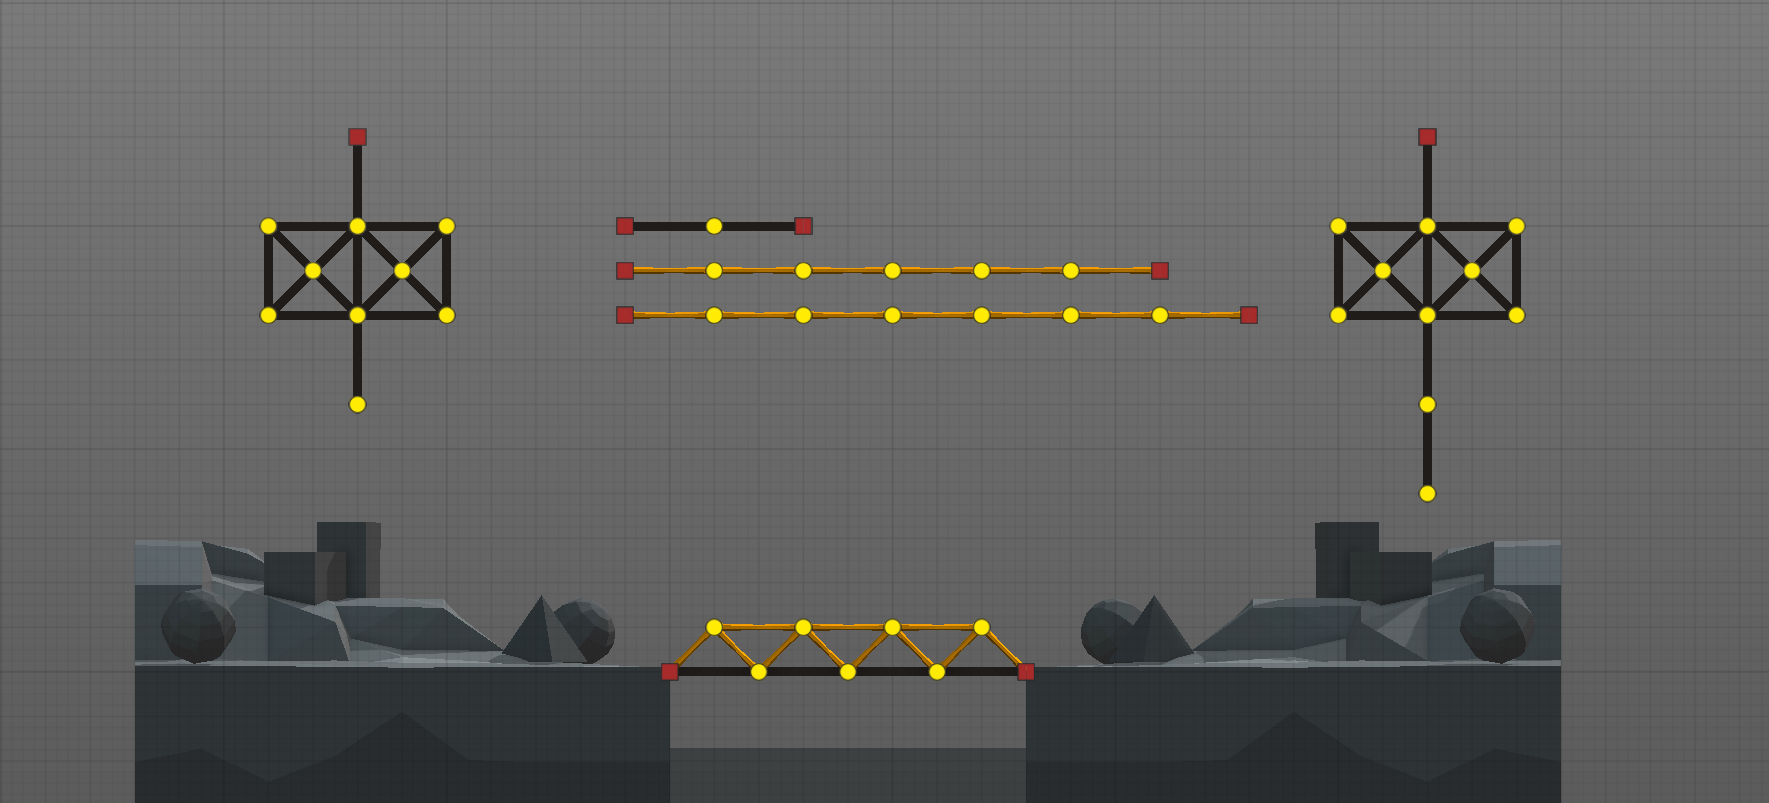
\includegraphics[width=\linewidth]{img/poly_tests.png}
    \end{minipage}\hfill
    \begin{minipage}{0.49\textwidth}
        \centering
        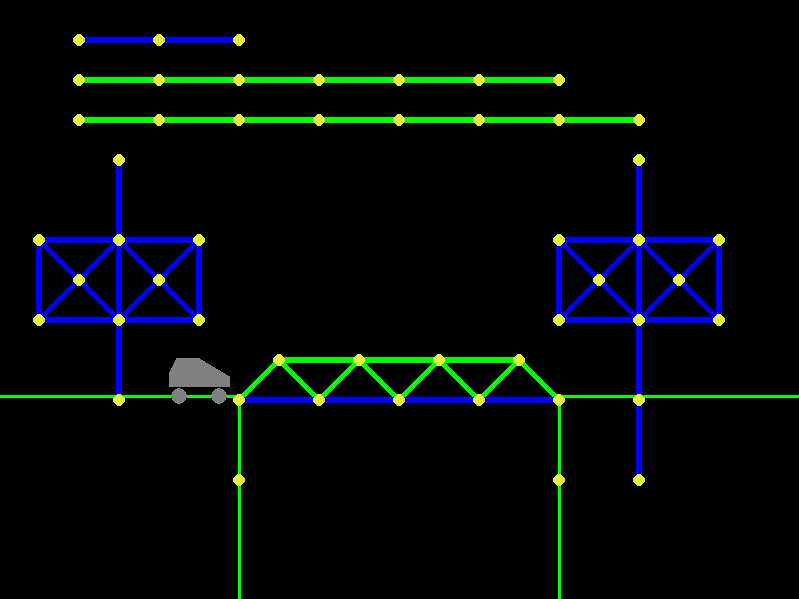
\includegraphics[width=\linewidth]{img/sim_tests.png}
    \end{minipage}
    \caption{Vizualizace testů ve hře polybridge (vlevo) a v simulaci (vpravo). Test č.1 nahoře uprostřed. Test č. 2 a 3 pod test č.1. Nalevo test č.4. Napravo test č.5. Most z 6. testu uprostřed. Vozidlo jede z levého břehu na pravý}
    \label{impl-fig:1}
\end{figure}

Naše implementace simulace ma $4$ různé parametry.
\begin{itemize}
    \item \emph{Hustota dřeva}: Hustota materiálů pro dřevo (\texttt{Box2D.b2Density}).
    \item \emph{Koeficient hustoty}: Násobek hustoty dřeva, který bude použit pro hustotu vozovky.
    \item \emph{Max. zatížení dřeva}: Maximální zatížení dřeva.
    \item \emph{Keoficient zatížení}: Násobek maximálního zatížení dřeva, který bude použit pro maximální zatížení vozovky.
\end{itemize}

Pro nalezení takových parametrů, které splní nejvíce testů jsme zvolili \textit{Random search} \cite{Random}. Prohledaná rozmezí těchto parametrů a jejich nejlepší nalezené hodnoty můžeme vidět v tabulce \ref{tab:1}. Bohužel se nám nepodařilo najít takové parametry, abychom splnili všechny. Rozhodli jsme se že $5.$ test vyřadíme.


\begin{table}[b!]
\centering
\begin{tabular}{l@{\hspace{1.5cm}}D{.}{,}{3}D{.}{,}{3}}
\toprule
\textbf{Parametr} & \multicolumn{1}{c}{\textbf{Rozmezí}} & \multicolumn{1}{c}{\textbf{Nalezená hodnota}$^a$} \\
\midrule
\emph{Hustota dřeva} & [0,01-3,01] & 1,348 \\
\emph{Max. zatížení dřeva} & [50,0-2050,0] & 765,0 \\
\emph{Koeficient hustoty} & [0,3-9,3] & 3,992 \\
\emph{Koeficient zatížení} & [0,1-5,1] & 0,821 \\
\bottomrule
\end{tabular}
\caption{Parametry pro simulaci, prohledávaná rozmezí a jejich nejlepší nalezená hodnoty.}\label{tab:1}
\footnotesize \textit{Pozn: $^a$Zaokrouhleno na 3 desetinná místa}
\end{table}


\subsection{Úrovně}

Jako testovací prostředí pro evoluční algoritmus jsme zvolili první $4$ úrovně z původní hry (viz obrázky \ref{impl-fig:2}, \ref{impl-fig:3}, \ref{impl-fig:4} a \ref{impl-fig:5}). Více úrovní jsme kvůli jejich komplexitě nezahrnuli.

\begin{figure}[ht]
    \centering
    \begin{minipage}{0.49\textwidth}
        \centering
        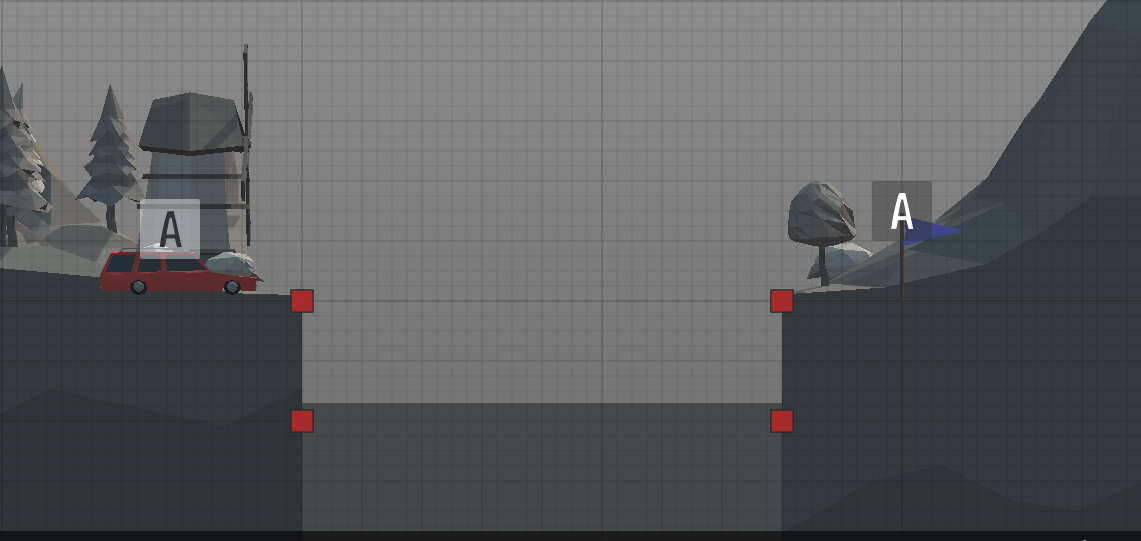
\includegraphics[width=\linewidth]{img/poly_lvl1.png}
    \end{minipage}\hfill
    \begin{minipage}{0.49\textwidth}
        \centering
        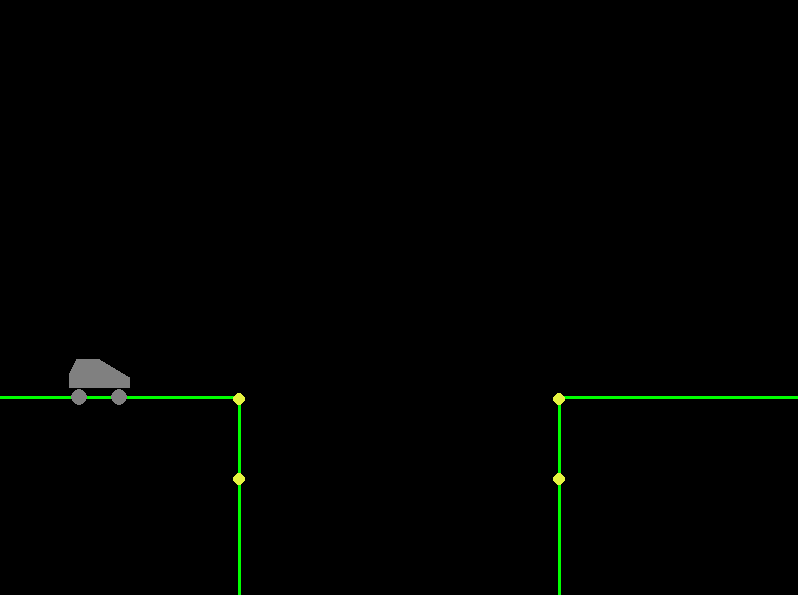
\includegraphics[width=\linewidth]{img/impl_lvl1.png}
    \end{minipage}
    \caption{Vizualizace $1.$ úrovně ve hře polybridge (vlevo) a v simulaci (vpravo)}
    \label{impl-fig:2}
\end{figure}

\begin{figure}[ht]
    \centering
    \begin{minipage}{0.49\textwidth}
        \centering
        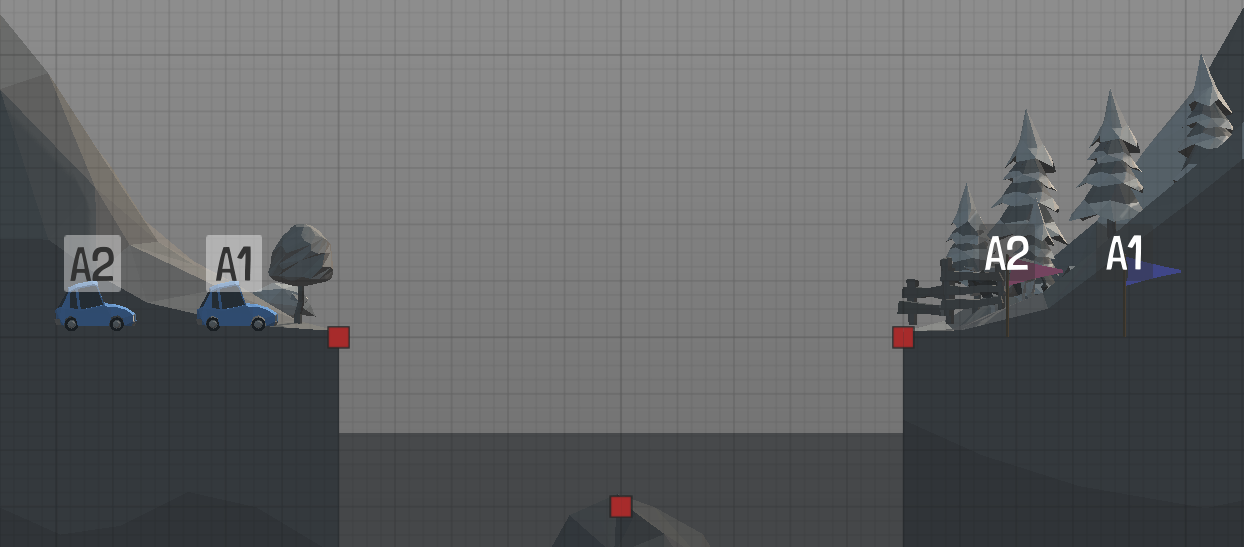
\includegraphics[width=\linewidth]{img/poly_lvl2.png}
    \end{minipage}\hfill
    \begin{minipage}{0.49\textwidth}
        \centering
        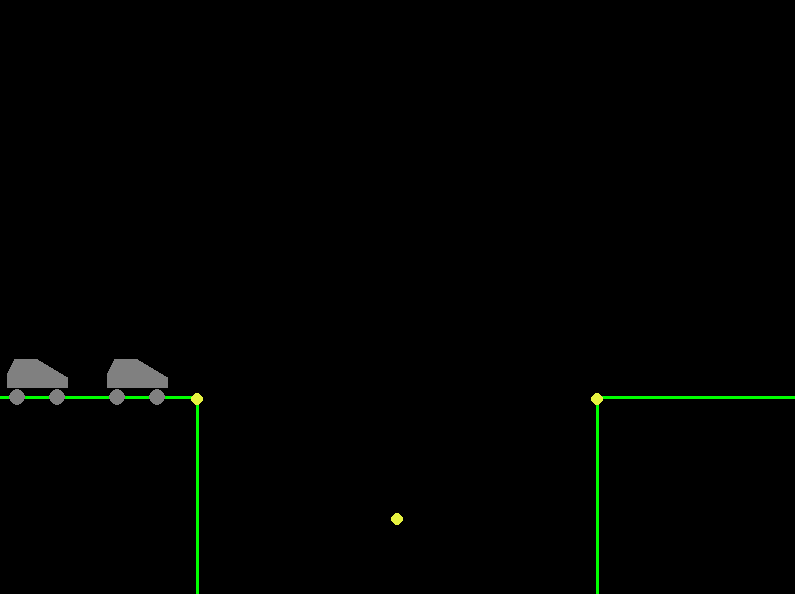
\includegraphics[width=\linewidth]{img/impl_lvl2.png}
    \end{minipage}
    \caption{Vizualizace $2.$ úrovně ve hře polybridge (vlevo) a v simulaci (vpravo)}
    \label{impl-fig:3}
\end{figure}

\begin{figure}[ht]
    \centering
    \begin{minipage}{0.49\textwidth}
        \centering
        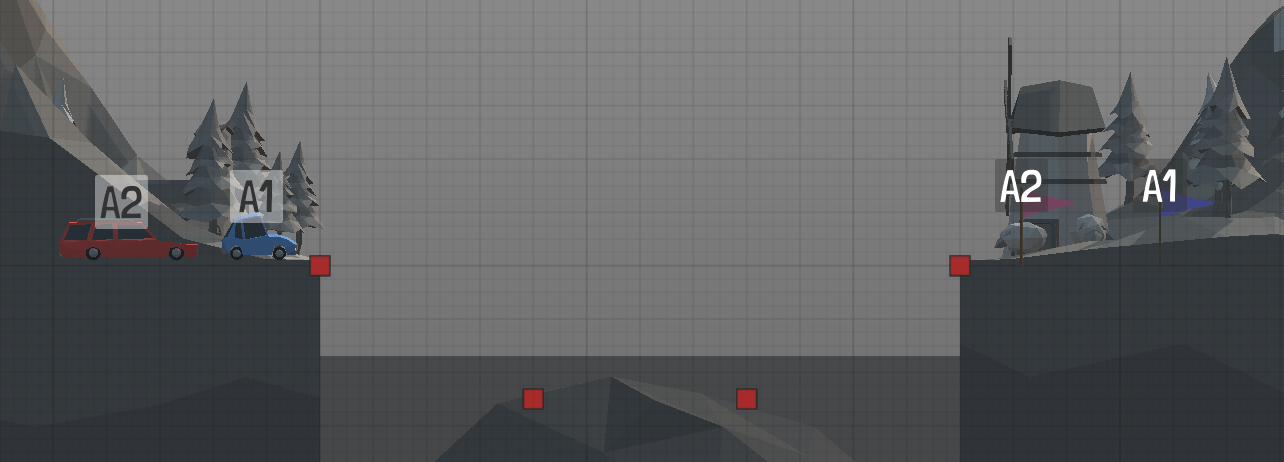
\includegraphics[width=\linewidth]{img/poly_lvl3.png}
    \end{minipage}\hfill
    \begin{minipage}{0.49\textwidth}
        \centering
        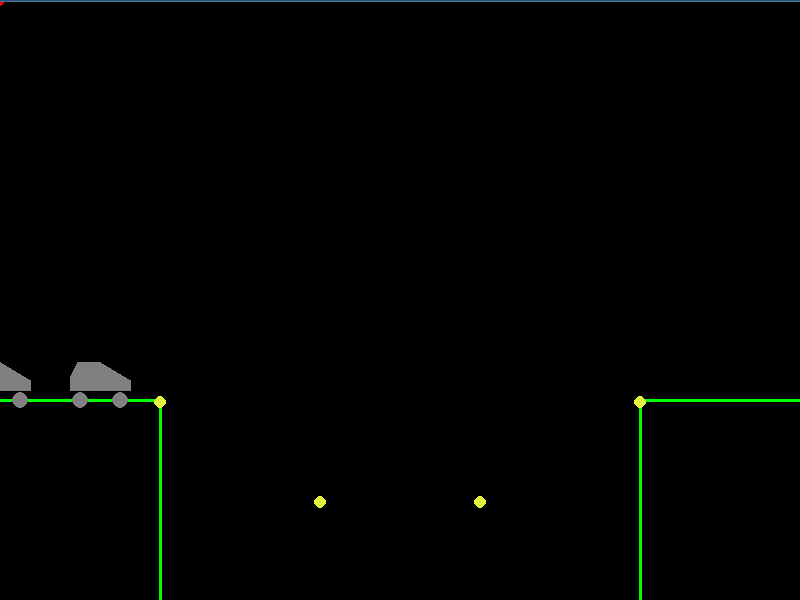
\includegraphics[width=\linewidth]{img/impl_lvl3.png}
    \end{minipage}
    \caption{Vizualizace $3.$ úrovně ve hře polybridge (vlevo) a v simulaci (vpravo)}
    \label{impl-fig:4}
\end{figure}

\begin{figure}[ht]
    \centering
    \begin{minipage}{0.49\textwidth}
        \centering
        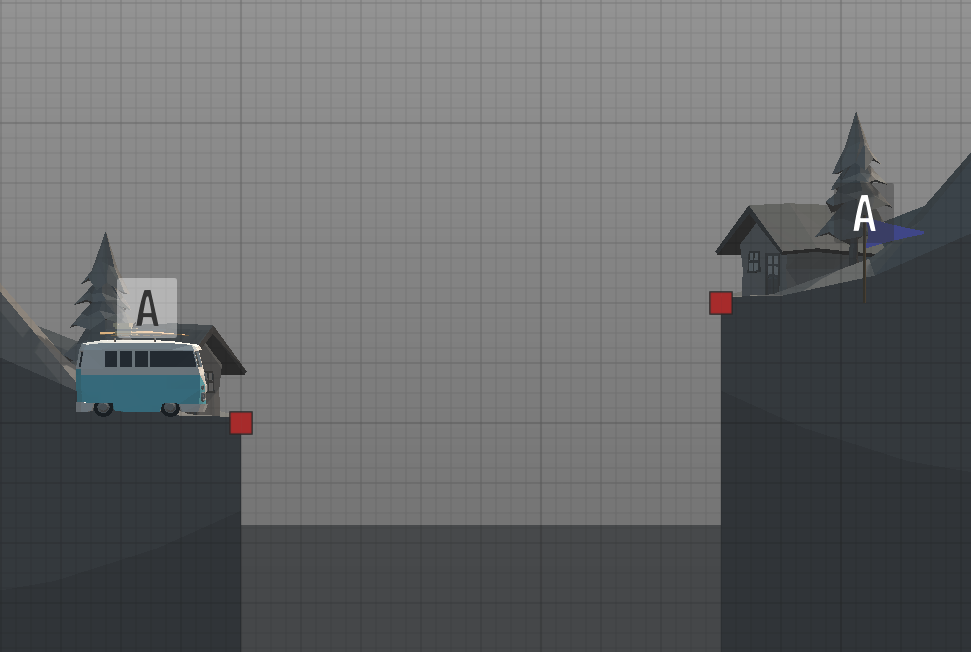
\includegraphics[width=\linewidth]{img/poly_lvl4.png}
    \end{minipage}\hfill
    \begin{minipage}{0.49\textwidth}
        \centering
        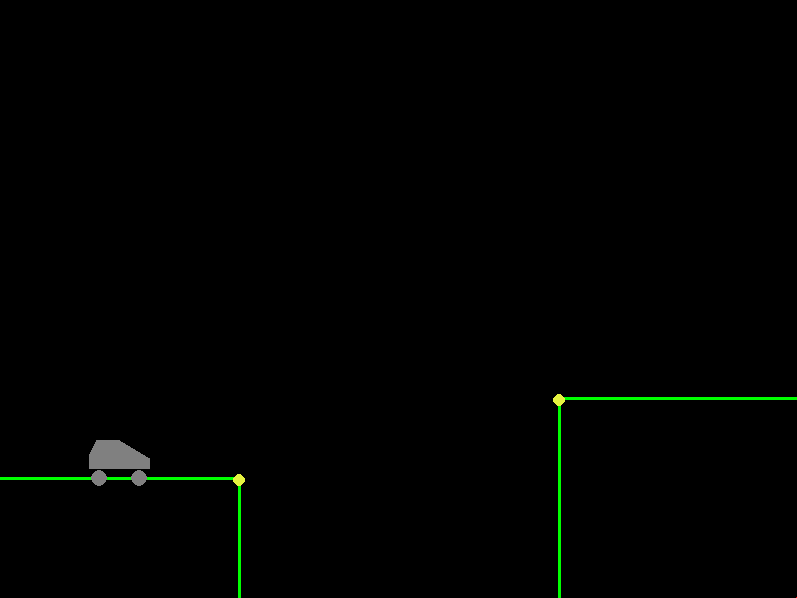
\includegraphics[width=\linewidth]{img/impl_lvl4.png}
    \end{minipage}
    \caption{Vizualizace $4.$ úrovně ve hře polybridge (vlevo) a v simulaci (vpravo)}
    \label{impl-fig:5}
\end{figure}


\section{Aplikace evolučních algoritmů}

V následující sekci ukážeme, jak jsme navrhli různé typy genetický operátorů. Budeme používat následující značení.
\begin{itemize}
    \item $l_{max}$ je maximální délka materiálu
    \item $T$ je množina všech materiálů, které můžeme použít (vozovka, dřevo, nic)
    \item $g$ je genom jedince, nebo také jeden konkrétní most
    \item $d_{min}(g)$ minimální vzdálenost vozidla od úrovní definovaného bodu na druhé straně řeky, které se podařilo dosáhnout v simulaci
    \item $cost(g)$ cena mostu $g$
\end{itemize}

Ve všech případech se snažíme optimalizovat dvě hodnoty a to jak daleko naše vozidlo dojelo a cenu mostu. V rámci algoritmu se tedy primárně snažíme maximalozovat $-d_{max}(g)$ a sekundárně $-cost(g)$.

Naše fitness funkce $f$ bude tedy udávaná dvojicí čísel. $$f(g) = (-d_{min}(g), -cost(g))$$

\subsection{Jednoduchý návrh}

Nejjednodušší návrh danému problému by mohl vypadat následovně. Reprezentace genu je vektor dvojic čísel $c \in \{([0, \dots, x_{max}] \times [0, \dots, y_{max}])\}^n$ kde $x_{max} \in \N$ a $y_{max} \in \N$ je šířka a výška úrovně a vektor $t \in T^n$. Most se pak z genomu postavíme následovně. Iterujeme přes všechny dvojice z $c$ a zároveň i přes materiály z $t$. Mezi bod tvořený současnou dvojicí a posledním bodem, na který jsme materiál přidali, se snažíme položit současný materiál. Pokud je současný bod od toho minulého příliš daleko tak jej přiblížíme aby jeho vzdálenost byla $l_{max}$. Na začátku jako poslední bod vybereme nejvyšší kotvu na levém břehu. Tímto způsobem se snažíme napodobit posloupnost kliknutí, které by hráč normálně provedl.

Jake mutaci jsme zvolili náhodné posunutí pozice kliknutí (bodu) o $\pm 1$ s pravděpodobností $\frac{1}{n}$ a náhodnou změnu materiálu s pravděpodobností $\frac{1}{n}$.

Jako křížení jsme použili jednobodové křížení vektoru $c$ a $t$ podle stejně zvoleného náhodného bodu. Jako selekci jsme zvolili turnajovou selekci.

Jak můžeme vidět v experimentu \ref{exp:2}, algoritmu se nedaří stavět příliš kvalitní mosty. Domníváme se, že by tomu tak je z následujících důvodů.

\begin{itemize}
    \item Z principu reprezentace jedince je nepravděpodobné, aby vznikaly krátké hrany, které mohou být klíčové pro kvalitní řešení.
    \item I malá mutace na začátku genu může mít velký vliv na celkovou strukturu mostu.
    \item Křížení v naší reprezentaci nedává smysl.
    \item Fitness funkce nevrací dobrou zpětnou vazbu o kvalitě jedince (viz. obrázek \ref{impl-fig:6})
\end{itemize}

\subsection{Polární kódování}

Kvůli tomu, jak jsme reprezentovali jedince v předchozím návrhu, je nepravděpodobné, že budou vznikat krátké hrany, které mohou být zásadní pro dobré řešení. To, že náhodně zvolíme blízko od od posledního kliknutí je méně pravděpodobné, než že zvolíme bod daleko. Proto jsme navrhli kódování genu, kde dvojce z vektoru $c$ představují délku a úhel přidaného materiálu $c \in \{([0, l_{max}] \times [0, 2 \pi])\}^n$. Vektor $t$ zůstává stejný jako v předchozím případě.

Jake mutaci jsme zvolili přepsání hodnoty z $c$ na novou náhodně zvolenou s pravděpodobností $\frac{1}{n}$ a náhodnou změnu materiálu s pravděpodobností $\frac{1}{n}$.

Křížení a selekci použijeme stejnou jako v předchozím případě.

\subsection{Vylepšená fitness funkce}

Jedním z problémů, se kterým se náš současný návrh potýká je ten, že naše fitness funkce moc dobře nerozlišuje, jak je dané řešení kvalitní. Na obrázku \ref{impl-fig:6} můžeme vidět dva různé jednice, kteří mají stejnou fitness, a v kvalitě se značně liší.


\begin{figure}[ht]
    \centering
    \begin{minipage}{0.49\textwidth}
        \centering
       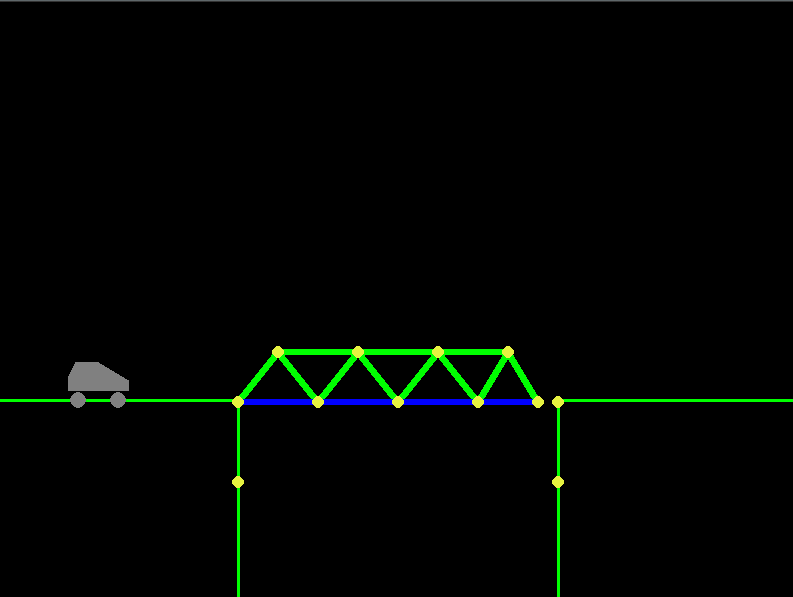
\includegraphics[width=\linewidth]{img/almost_good_bridge.png}
    \end{minipage}\hfill
    \begin{minipage}{0.49\textwidth}
        \centering
        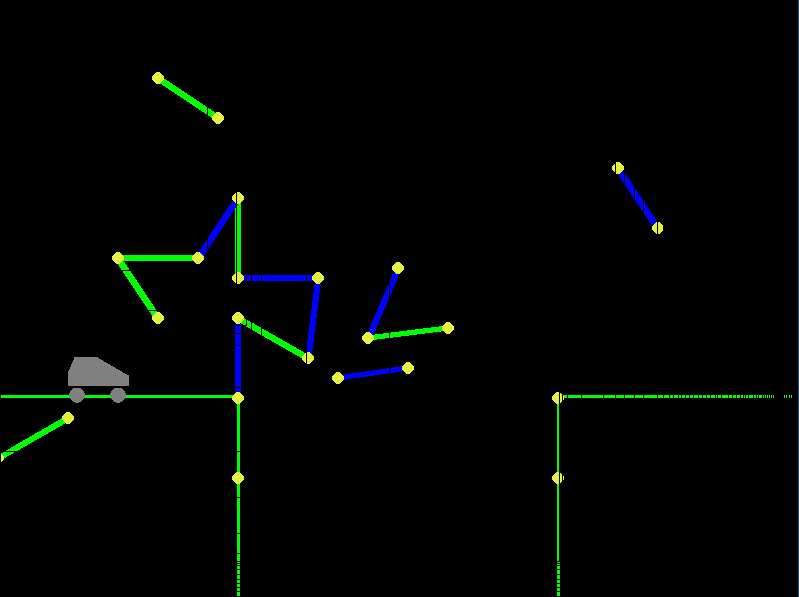
\includegraphics[width=\linewidth]{img/bad_bridge.png}
    \end{minipage}
    \caption{Dva mosty se stejnou fitness, ale rozdílných kvalit}
    \label{impl-fig:6}
\end{figure}

Navrhli jsme proto dvě různé penalizace, které můžeme do fitness zapojit.

\begin{itemize}
    \item Penalizace za umisťování materiálů, který se nespojí s další materiálem. Lépe propojený most by měl mít lepší stabilitu.
    \item Penalizace za všechny kotvy, které jedinec nepoužil. V praxi použijem vzdálenost každého kliknutí ke všem nepoužitým kotvám. Most který používá více kotev by měl být stabilnější.
\end{itemize}

Nová fitness funkce pak vypadá následovně. $$f(g) = (-d_{min}(g) + \alpha \cdot mat + \beta \cdot anch, -cost(g))$$ Koeficinety $\alpha, \beta \in \R$ značí váhu penalizace a $mat, anch$ jsou hodnoty penalizace za nespojený materiál a nevyužité kotvy.

Použijeme stejnou selekci, mutaci a reprezentaci jedince jako v předchozím návrhu.

\subsection{Měnící se fitness}

V rámci našeho přístupu jsme narazili na specifický problém spojený se stabilitou mostu. Spočívá v tom, že dokud není most zcela dokončen, nedosahuje potřebné stability, které je potřeba pro přejetí vozidlem. Abychom se s tímto omezením vypořádali, rozhodli jsme se pro zjednodušení problému a využití techniky zvané \emph{inkrementální evoluční alogritmus} navrhnuté ve článku Mansouryho Nashaata et al. \cite{IGA}. Na začátku experimentu proto začínáme s břehy blíže umístěnými k sobě a jakmile dosáhneme dostatečně nízké průměrné fitness v celé populaci, vzdálenost postupně zvětšujeme, dokud nedosáhneme vzdálenosti definové úrovní. 

Použijeme stejnou selekci, mutaci a reprezentaci jedince jako v předchozím návrhu.

\subsection{Grafové kódování}

V této části bychom chtěli představit odlišný způsob, jak kódovat jednotlivce. Naše dosavadní kódování značně trpí tím, že je nepravděpodobné aby, se v jednom bodě spojilo více, než dva kusy materiálu. Tento problém se pokusíme vyřešit tím, že jedince budeme kódovat jako graf, tedy pomocí vrcholů a hran. To v praxi znamená, že gen jedince se skládá z množiny vrcholů $V$, množiny hran $E \subseteq V \times V$, funkce $\sigma_v : V \rightarrow \R^2$ která je projekcí $V$ do roviny a $\sigma_e : E \rightarrow T$. Naše navržené genetické operátory vypadají následovně.

\begin{itemize}
    \item \textbf{inicializace}: Do $V$ přidáme všechny kotvy z úrovně. Náhodně vybereme materiál $t \in T$, vrchol $v_1 \in V$, úhel $\varphi$ a délku $0 < l < l_{max}$. Vytvoříme nový vrchol $v_2$ a vložíme jej do $V$. Upravíme $\sigma_v$ tak, že $v_2$ se promítne na bod ve vzdálenosti $l$ a pod úhlem $\varphi$ od $\sigma_v(v_1)$. Vytvoříme novou hranu $(v_1, v_2)$ a přidáme jí do $E$ a zároveň upravíme $\sigma_e$ tak, že $\sigma_e((v_1, v_2)) = t$. Opakujeme dokud nevytvoříme $n$ nových vrcholů. Následně náhodně volíme dva vrcholy $v_1, v_2 \in V$. Pokud $||\sigma_v(v_1) - \sigma_v(v_2)|| < l_{max}$ vytvoříme novou hranu $(v_1, v_2)$ a přidáme do $E$. Upravíme $\sigma_e((v_1, v_2)) = t$ pro náhodně zvolené $t \in T$. Opakujeme $2n$-krát.
    \item \textbf{mutace}: Budeme rozlišovat mutaci pro vrcholy a mutaci pro hrany. Mutace pro vrcholy upraví $\sigma_v$ tak, že projekci vrcholu $v \in V$ přemístí na náhodně zvolený bod z $\{ x \in \R^2 | \forall v_2 \in Adj(v_1), ||x - \sigma_v(v_2)|| < l_{max}\}$ kde $Adj(v_1) = \{v \in V | (v_1, v) \in E\}$. Jinými slovy náhodně posumeme vrchol $v$ tak, aby nebyl příliš daleko od žádného vrcholu s nímž byl $v$ spojen hranou. Mutace pro hrany může hranu přidat, odebrat jí nebo změnit $\sigma_e$ náhodné hrany na jiný typ materiálu.
    \item \textbf{křížení}: Dva jedince můžeme skřížit následovně. Nechť $V_1, E_1$ je množina všech vrcholů a hran prvního z rodičů a $V_2, E_2$ druhého. Nechť $\sigma_{v_p}$ je spojení $\sigma_v$ funkcí obou rodičů a $\sigma_{e_p}$ spojení $\sigma_e$ funkcí obou rodičů. Zvolíme náhodně hranici $min\{\sigma_{v_p}(v)_x | v \in V_1 \cup V_2\} < p_x < max\{\sigma_{v_p}(v)_x | v \in V_1 \cup V_2\}$. Nechť $L = \{ v | v \in V_1, \sigma_{v_p}(v)_1 < p_x\}$ a $R = \{ v | v \in V_2, \sigma_{v_p}(v)_1 > p_x\}$. Vrcholy genu potomka pak budou z $V_p = R + L$ a hrany $E_p = (E_1 + E_2) \cap V_p \times V_p$, kterým navíc přidáme všechny $(v_1, v_2), v_1 \in R, v_2 \in L, ||\sigma_{v_p}(v_1) - \sigma_{v_p}(v_2)|| < l_{max}$ s pravděpodobností $\alpha$. $\sigma_v$ potomka bude $\sigma_{v_p}$ a stejně tak pro $\sigma_e$. Příklad takové mutace můžeme vidět na obrázku \ref{impl-fig:8}
\end{itemize}

\begin{figure}[ht]
    \centering
    \begin{minipage}{0.24\textwidth}
        \centering
        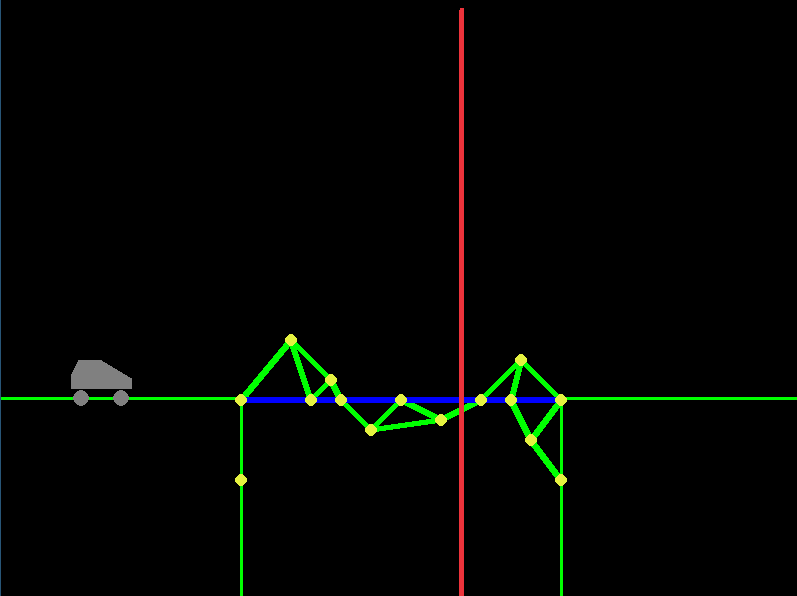
\includegraphics[width=\linewidth]{img/bridge_p1.png}
    \end{minipage}\hfill
    \begin{minipage}{0.24\textwidth}
        \centering
        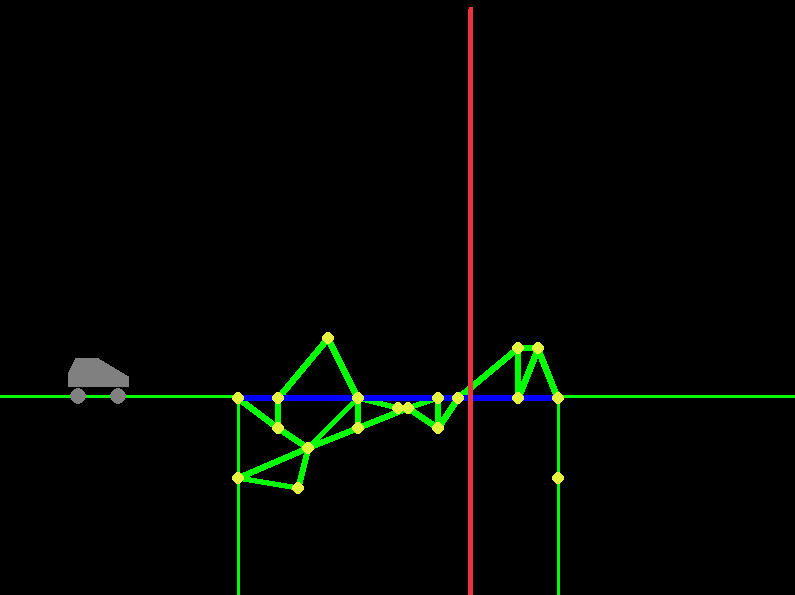
\includegraphics[width=\linewidth]{img/bridge_p2.png}
    \end{minipage}
    \begin{minipage}{0.24\textwidth}
        \centering
        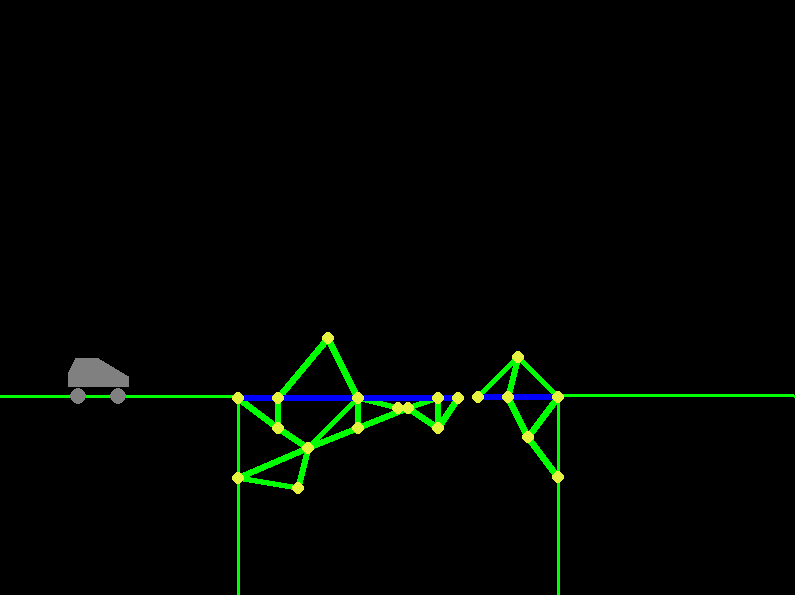
\includegraphics[width=\linewidth]{img/bridge_crossed.png}
    \end{minipage}
    \begin{minipage}{0.24\textwidth}
        \centering
        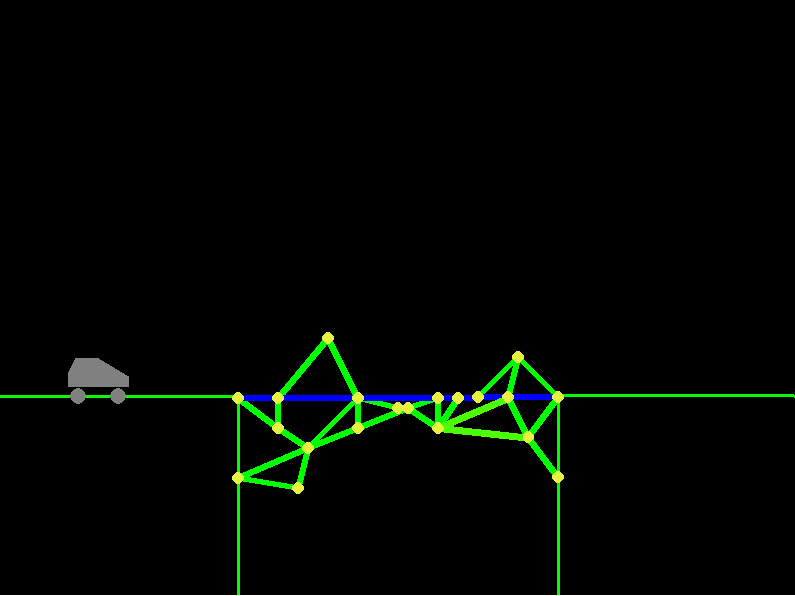
\includegraphics[width=\linewidth]{img/bridge_sups.png}
    \end{minipage}
    \caption{Příklad křížení dvou rodičů. Na 1. a 2. obrázku zleva jsou rodiče. Hranice pro náhodné křížení je vyznačena červenou čárou. Na 2. obrázku zprava křížení částí mosty. Na nejpravějším obrazku překžížení s vystužením}
    \label{impl-fig:8}
\end{figure}

Jako selekci použijeme turnajovou selekci.

\subsection{Lepší inicializace}

Do našeho algoritmu můžeme ještě zahrnout jednu z nejsilnějších techni pro evoluční algoritmy a to použití \textit{domain-specific} znalostí \cite{PASSONE2006192}. I když ještě nevíme, jak bude optimální most vypadat, dokážeme obecným způsobem navrhnout most, který sice nebude optimální, ale bude lepší, než náhodně umístěný materiál. Z tohoto důvodu jsme implementovali postup podobný tomu, který navrhli Hugo Lispector ve své diplomové práci \cite{Lispector2022}. Tento postup se skládá ze tří kroků.

\begin{enumerate}
    \item \textbf{Vytvoření vozovky}: Nejprve pro vozidlo vytvoříme vozovku a to tím způsobem, spojíme levý a pravý břeh vozovkami a náhodné délce.
    \item \textbf{Vytvoření opor}: Následně pro každou ještě nevyužitou kotvu vyberem jeden spojový kloub z předchozího kroku a spojíme je dřevěnými díly o náhodné délce.
    \item \textbf{Zpevnění}: Nakonec pro každý přidaný materiál náhodně vybereme nový bod tak, abychom jej mohli spojit jedním dílem dřeva se začátkem a koncem tohoto materiálu a navíc bod spojíme se všemi ostatními bodu v blízkém okolí s pravděpodobností $\omega$.
\end{enumerate}

Vizualizaci těchto tří kroků můžeme vidět na obrázku \ref{impl-fig:7}

\begin{figure}[ht]
    \centering
    \begin{minipage}{0.32\textwidth}
        \centering
        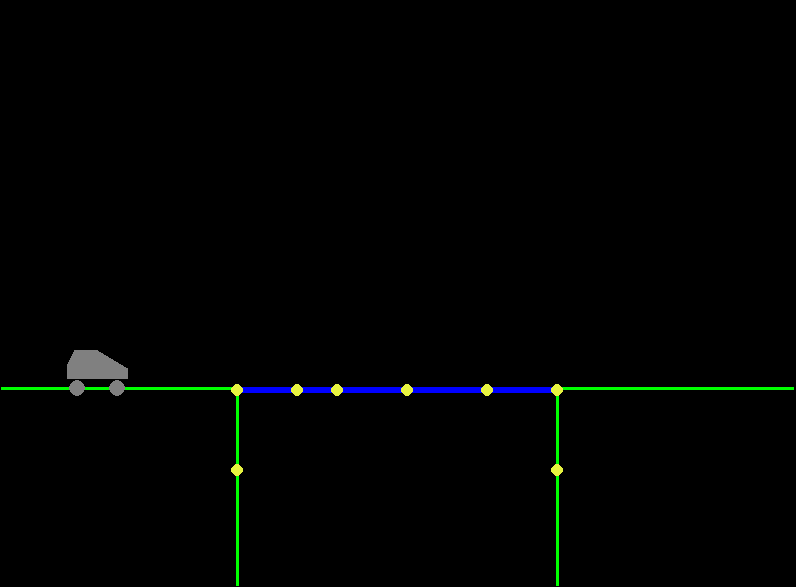
\includegraphics[width=\linewidth]{img/better_init1.png}
    \end{minipage}\hfill
    \begin{minipage}{0.32\textwidth}
        \centering
        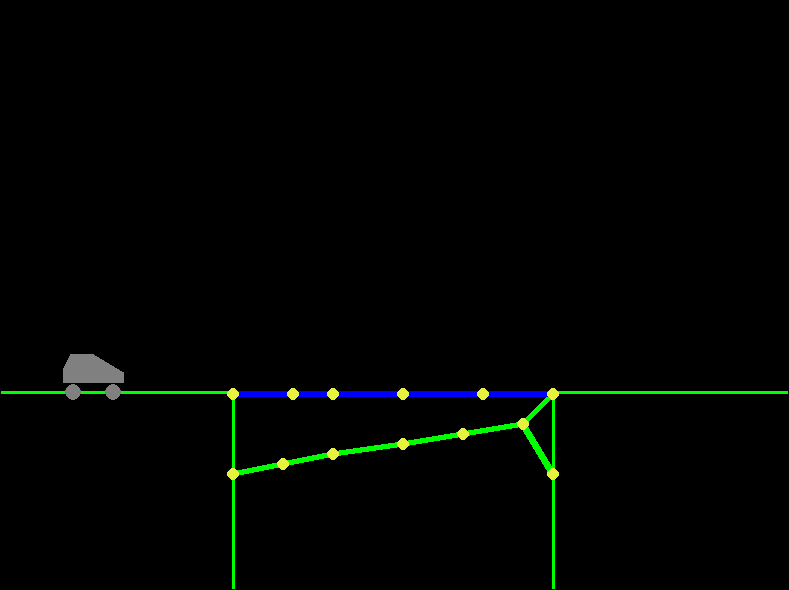
\includegraphics[width=\linewidth]{img/better_init2.png}
    \end{minipage}
    \begin{minipage}{0.32\textwidth}
        \centering
        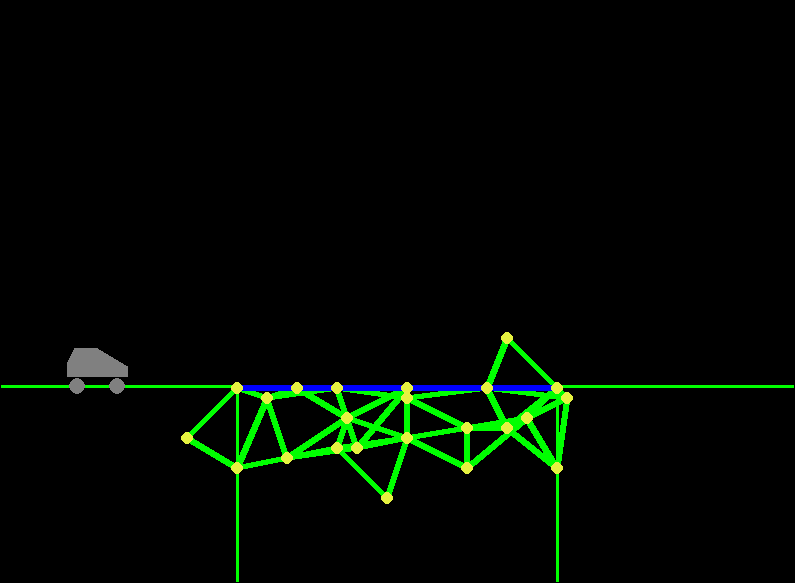
\includegraphics[width=\linewidth]{img/better_init3.png}
    \end{minipage}
    \caption{Výtváření jedince pomocí lepší inicializace. Krok \textbf{Vytvoření vozovky} vlevo, krok \textbf{Vytoření opor} uprostřed a krok \textbf{Zpevění} s $\omega = 1$ vpravo}
    \label{impl-fig:7}
\end{figure}

Použijeme selekci, křížení a mutaci z přechozího návrhu.

\chapter{Experimenty}

\section{Jednoduchý příklad s batohem}
\begin{figure}[p]\centering
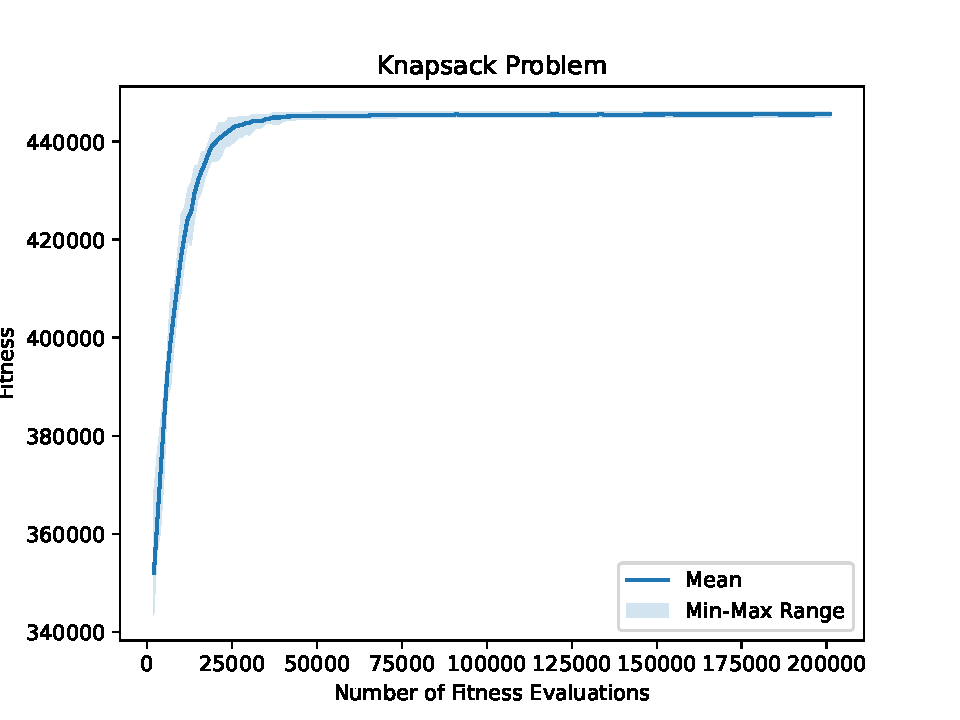
\includegraphics[width=140mm, height=140mm]{img/knap}
\caption{Popisek?}
\label{exp:1}

\end{figure}


\section{Naivní přístup}
\begin{figure}[p]\centering
\includegraphics[width=140mm, height=140mm]{img/simple}
\caption{Popisek?}
\label{exp:2}
\end{figure}


\section{Agent s polárním kódováním}
\begin{figure}[p]\centering
\includegraphics[width=140mm, height=140mm]{img/polar}
\caption{Popisek?}
\label{exp:3}
\end{figure}


\section{Vylepšená fitness funkce}
\begin{figure}[p]\centering
\includegraphics[width=140mm, height=140mm]{img/impolar}
\caption{Popisek?}
\label{exp:4}
\end{figure}


\section{Populace s eliticismem}
\begin{figure}[p]\centering
\includegraphics[width=140mm, height=140mm]{img/elit}
\caption{Popisek?}
\label{exp:5}
\end{figure}


\section{Stěžující se fitness}
\begin{figure}[p]\centering
\includegraphics[width=140mm, height=140mm]{img/inc}
\caption{Popisek?}
\label{exp:6}
\end{figure}


\chapter*{Závěr}

\addcontentsline{toc}{chapter}{Závěr}



%%% Seznam použité literatury
%%% Seznam použité literatury (bibliografie)
%%%
%%% Pro vytváření bibliografie používáme bibTeX. Ten zpracovává
%%% citace v textu (např. makro \cite{...}) a vyhledává k nim literaturu
%%% v souboru literatura.bib.
%%%
%%% Příkaz \bibliographystyle určuje, jakým stylem budou citovány odkazy
%%% v textu. V závorce je název zvoleného souboru .bst. Styly plainnat
%%% a unsrt jsou standardní součástí latexových distribucí. Styl czplainnat
%%% je dodáván s touto šablonou a bibTeX ho hledá v aktuálním adresáři.

\bibliographystyle{czplainnat}    %% Autor (rok) s českými spojkami
% \bibliographystyle{plainnat}    %% Autor (rok) s anglickými spojkami
% \bibliographystyle{unsrt}       %% [číslo]

\renewcommand{\bibname}{Seznam použité literatury}

%%% Vytvoření seznamu literatury. Pozor, pokud jste necitovali ani jednu
%%% položku, seznam se automaticky vynechá.

\bibliography{literatura}

%%% Kdybyste chtěli bibliografii vytvářet ručně (bez bibTeXu), lze to udělat
%%% následovně. V takovém případě se řiďte normou ISO 690 a zvyklostmi v oboru.

% \begin{thebibliography}{99}
%
% \bibitem{lamport94}
%   {\sc Lamport,} Leslie.
%   \emph{\LaTeX: A Document Preparation System}.
%   2. vydání.
%   Massachusetts: Addison Wesley, 1994.
%   ISBN 0-201-52983-1.
%
% \end{thebibliography}


%%% Obrázky v práci
%%% (pokud jich je malé množství, obvykle není třeba seznam uvádět)
\listoffigures

%%% Tabulky v práci (opět nemusí být nutné uvádět)
%%% U matematických prací může být lepší přemístit seznam tabulek na začátek práce.
\listoftables

%%% Použité zkratky v práci (opět nemusí být nutné uvádět)
%%% U matematických prací může být lepší přemístit seznam zkratek na začátek práce.
\chapwithtoc{Seznam použitých zkratek}

%%% Součástí doktorských prací musí být seznam vlastních publikací
\ifx\ThesisType\TypePhD
\chapwithtoc{Seznam publikací}
\fi

%%% Přílohy k práci, existují-li. Každá příloha musí být alespoň jednou
%%% odkazována z vlastního textu práce. Přílohy se číslují.
%%%
%%% Do tištěné verze se spíše hodí přílohy, které lze číst a prohlížet (dodatečné
%%% tabulky a grafy, různé textové doplňky, ukázky výstupů z počítačových programů,
%%% apod.). Do elektronické verze se hodí přílohy, které budou spíše používány
%%% v elektronické podobě než čteny (zdrojové kódy programů, datové soubory,
%%% interaktivní grafy apod.). Elektronické přílohy se nahrávají do SISu.
%%% Povolené formáty souborů specifikuje opatření rektora č. 72/2017.
%%% Výjimky schvaluje fakultní koordinátor pro zavěrečné práce.
\appendix
\chapter{Přílohy}

\section{První příloha}

\end{document}
